\section{基于优化方法的状态估计}

目前绝大多数的SLAM算法通过集束优化\citep{triggs1999bundle}(Bundle Adjustment,BA)方法来对状态进行估计在传统的视觉SfM算法中,集束优化是指通过联合优化所有的视觉观测误差来同时求解最优的相机位姿状态和三维点状态的方法。而对于使用了更多传感器的SLAM系统,除了三维点和位姿状态,集束优化算法还需要实时地、持续对系统的其他状态比作出估计。对于视觉惯性SLAM,集束优化通常会通过联合优化所有的视觉观测和惯性观测来同时求解相机或IMU的位姿、速度以及IMU的bias状态。

\subsection{基于图优化的状态估计}

图优化方法是分析并求解SLAM后端状态估计问题的常用工具。最早在机器人领域,为了解决多段激光传感器数据额融合时的全局一致性问题,\citep{lu1997globally,lu1997robot}提出了基于位姿图的优化方法。\citeauthor{thrun2006graph}在此基础上进一步提出了GraphSLAM\citep{thrun2006graph},使用由位姿状态和三维点状态以及它们之间的约束构成的因子图来描述集束优化问题。因子图可以很直观地描述集束优化问题中状态和约束之间的关联,有助于分析集束优化问题的各种性质。经过长时间的发展,图优化方法已经成为SLAM领域的经典方法。

\begin{figure}[htb!]
    \centering
    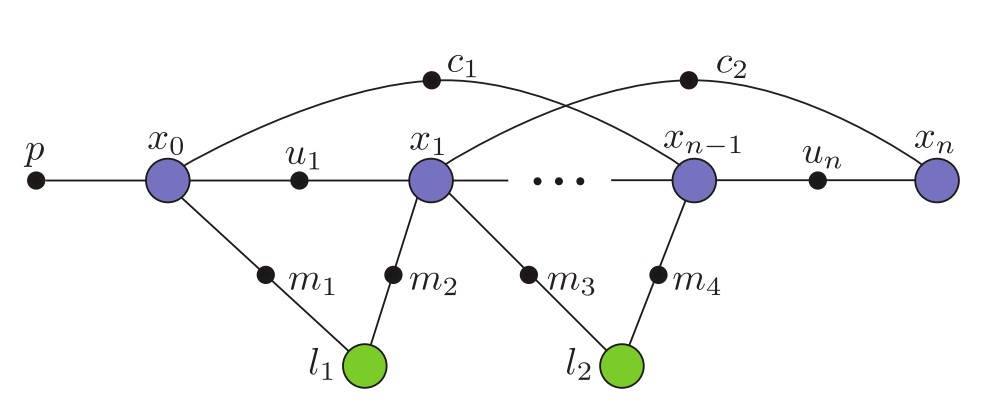
\includegraphics[width=.8\textwidth]{figs/isam_factor_graph.png}
    \caption{因子图示例\citep{kaess2012isam2}:紫色节点代表位姿状态,绿色节点代表三维点状态,黑色节点代表状态之间的约束因子。}
    \label{fig:isam_factor_graph}
\end{figure}

图\ref{fig:isam_factor_graph}展示了一类常见的因子图结构。按照图示的例子,一个SLAM问题中可能存在的约束有状态变量的先验约束$p$,相邻状态之间的相对位姿约束$u_1 \dots u_n$,非相邻状态之间的回路闭合约束$c_1,c_2$以及视觉观测约束$m_1 \dots m_4$等。而求解完整集束优化的过程就相当于最大化整个因子图中的所有约束的集合$\mathcal{Z}$关于所有状态集合$\mathcal{X}$的联合条件概率:
\begin{equation}
    P(\mathcal{Z}|\mathcal{X}) = \prod_{f_i\in\mathcal{Z}} P(f_i(\mathcal{X}_i))
\end{equation}
其中$\mathcal{X}_i$代表所有与约束节点$f_i$相邻的状态节点。通常会假设这是一个高度非线性系统,并且所有的约束$f_i$的噪声服从高斯分布$f_i\sim\mathcal{N}(\mu_i, \sigma_i^2)$。这样的的概率最大化问题通常被转化为非线性最小二乘(Non-linear Least Squares,NLS)问题来求解:
\begin{equation}
\begin{aligned}
    \mathcal{X}^\star &= \mathop{\arg\max}_{\mathcal{X}}
                         \prod_{f_i\in\mathcal{Z}} P(f_i(\mathcal{X}_i)) \\
                      &= \mathop{\arg\min}_{\mathcal{X}}
                         \sum_{f_i\in\mathcal{Z}} \frac{1}{2}
                         \lVert f_i(\mathcal{X}_i)) \rVert_{\sigma_i^2}^2
\end{aligned}
\end{equation}

\subsection{非线性最小二乘}

非线性最小二乘问题难以被直接求解,通常要使用迭代求解的方法来逼近局部最优解。如果变量的初值在全局最优解的附近,则一般可以使用牛顿法(Newton's method)迭代求解。如下给出了而一个典型的非线性最小二乘问题的形式:
\begin{equation}
\begin{aligned}
    \bm{x}^\star &= \mathop{\arg\min}_{\bm{x}} F(\bm{x}) \\
                 &= \mathop{\arg\min}_{\bm{x}}
                    \frac{1}{2} \Vert \mathbf{f}(\bm{x}) \Vert^2
\end{aligned}\label{eq:nlls}
\end{equation}
其中变量$\bm{x}\in\mathbb{R}$,$\mathbf{f}(\cdot)$为关于变量$\bm{x}$的非线性函数,即目标函数。

在局部最优解附近,最小化能量函数$F(\cdot)$等同于求解其梯度函数$\bm{g}(\cdot)$的零点(对于线性的函数则为唯一的零点),即:
\begin{equation}
    \bm{g} \doteq \nabla F = \begin{bmatrix}
        \frac{\partial F}{\partial x_1} &
        \frac{\partial F}{\partial x_2} &
        \cdots &
        \frac{\partial F}{\partial x_n}
    \end{bmatrix}^\top = \bm{0}
\end{equation}

采用牛顿法求解上述零点问题,记梯度函数$\bm{g}(\cdot)$的一阶导数为海森矩阵(Hessian matrix):
\begin{equation}
    \mathrm{H} \doteq \begin{bmatrix}
        \frac{\partial^2 F}{\partial x_1^2} &
        \frac{\partial^2 F}{\partial x_1 \partial x_2} &
        \cdots & \cdots &
        \frac{\partial^2 F}{\partial x_1 \partial x_n} \\
        %
        \frac{\partial^2 F}{\partial x_2 \partial x_1} &
        \frac{\partial^2 F}{\partial x_2^2} &
        & &
        \frac{\partial^2 F}{\partial x_2 \partial x_n} \\
        %
        \vdots & & \ddots & & \vdots \\
        \vdots & & & \ddots & \vdots \\
        %
        \frac{\partial^2 F}{\partial x_n \partial x_1} &
        \frac{\partial^2 F}{\partial x_n \partial x_2} &
        \cdots & \cdots &
        \frac{\partial^2 F}{\partial x_n^2}
    \end{bmatrix}
\end{equation}
求解如下线性系统:
\begin{equation}
    \bm{x} = -\mathrm{H} \enspace\setminus\enspace \bm{g}
    \label{eq:linsys}
\end{equation}

线性的问题中,当矩阵$\mathrm{H}$为正定矩阵时, 给定任意初值$\bm{x}$(这里选择了初值为$\bm{0}$)只需一步就可解得式\eqref{eq:nlls}的全局最优解。而对于非线性的情况,则需要多次迭代才能解得局部最优解。

\subsection{高斯-牛顿法}\label{sec:gn}

对于非线性最小二乘问题,牛顿法中计算函数$F(\cdot)$的准确海森矩阵$\mathrm{H}$的代价往往很大,甚至没有闭解。一些算法会寻求使用近似方法计算每次迭代的海森矩阵,比如拟牛顿法\citep{tingleff2004methods}(Qausi-Newton method)。拟牛顿法适用于一般的最小化问题,而对于非线性最小二乘问题,通常可以高斯-牛顿法(Gauss-Newton method)求解。高斯-牛顿法是用于求解非线性最小二乘问题的经典迭代算法,也是众多其他迭代算法的基础。

依然考虑非线性最小二乘问题\eqref{eq:nlls},使用高斯-牛顿法迭代求解,首先要给定变量的初值$\bm{x}=\bm{x}_0$。对其在当前点处进行泰勒展开,并忽略高阶项,可得目标函数$\mathbf{f}(\cdot)$在$\bm{x}_0$处的线性近似:
\begin{equation}
    \mathbf{f}(\bm{x}_0+\bm{\delta}) \simeq \mathbf{f}_0 + \mathrm{J}\bm{\delta}
\end{equation}
其中$\mathrm{J}\in\mathbb{R}^{m \times n}$是目标函数$\mathbf{f}(\cdot)$在$\bm{x}_0$处的雅各比矩阵(Jacobian)。式\eqref{eq:nlls}被转化为局部$\bm{x}_0$处的线性最小二乘子问题
\begin{equation}
    \bm{\delta}_{gn} =
        \min_{\bm{\delta}} \frac{1}{2}
        \Vert \mathbf{f}_0 + \mathrm{J}\bm{\delta} \Vert^2
    \label{eq:lls}
\end{equation}
使用牛顿法求解这个线性最小二乘子问题,构建正规方程(normal equation)并求解,可得高斯-牛顿法一次迭代的结果:
\begin{equation}
    \bm{\delta}_{gn} =
        -\left( \mathrm{J}^\top\mathrm{J} \right)
        \enspace\setminus\enspace
        \left( \mathrm{J}^\top\mathbf{f}_0 \right)
    \label{eq:normal_eq}
\end{equation}
将此结果更新至变量:$\bm{x}\leftarrow\bm{x}_0+\bm{\delta}$,然后不断重复以上过程,直至结果收敛。

式\eqref{eq:normal_eq}和\eqref{eq:linsys}的形式类似,也可以认为高斯-牛顿法和牛顿法的最大区别就是高斯-牛顿法使用了$\mathrm{J}^\top\mathrm{J}$来近似海森矩阵$\mathrm{H}$。

\subsection{信赖域方法}

除了高斯-牛顿法之外,还有一种经典的求解非线性最小二乘优化的算法:莱文贝格-马夸特(Levenberg-Marquardt,LM)法。它也被认为是带有阻尼因子的高斯-牛顿法,也是信赖域方法(trust region method)的前身\citep{jorge2006numerical}。

众所周知,一般的VO算法中,尺度是不可观测的(unobservable)——在VO的状态估计中,对全局所有的三维点坐标和相机位置进行统一的缩放,不会引起重投影误差的改变(在不考虑数值误差的情况下)。从求解VO集束优化问题的角度来看,这一性质造成了在直接使用高斯-牛顿法时海森矩阵的秩亏现象,即矩阵$\mathrm{J}^\top\mathrm{J}$为半正定的情况。此时直接使用矩阵分解求逆的方法求解线性最小二乘子问题就会得到数值不稳定的结果,比如解得的步长在某个方向过大等。

\subsubsection*{莱文贝格方法}

针对这一情况,莱文贝格在基础的高斯-牛顿法中引入了对迭代步长的直接约束,将原先每次迭代的线性最小二乘子问题改写为:
\begin{equation}
    \bm{\delta}_{l} =
        \mathop{\min}_{\bm{\delta}} \frac{1}{2}
        \left(
            \Vert \mathbf{f}_0 + \mathrm{J}\bm{\delta} \Vert^2 +
            \mu \Vert \bm{\delta} \Vert^2
        \right), \quad \mu > 0
\end{equation}
这样一来,原先高斯-牛顿法求解的正规方程就变成了
\begin{equation}
    \bm{\delta}_l =
        -\left( \mathrm{J}^\top\mathrm{J}+\mu\mathrm{I} \right)
        \enspace\setminus\enspace
        \left( \mathrm{J}^\top\mathbf{f}_0 \right)
    \label{eq:levenberg}
\end{equation}
其中的$\mu$就是所谓的阻尼因子(damping factor)。

阻尼因子控制住了每次迭代计算的步长的模。通常阻尼因子$\mu$具备下面三个性质\citep{tingleff2004methods}:
\begin{enumerate}
    \item 对于任意的$\mu>0$,海森矩阵$(\mathrm{J}^\top\mathrm{J}+\mu\mathrm{I})$正定,这一点保证了求得的步长$\bm{\delta}$处于能量下降的方向;
    \item 当$\mu\to\infty$时,求得的步长$\bm{\delta}$接近于梯度下降方向$-\frac{1}{\mu}\mathrm{J}^\top\mathbf{f}(\bm{x})$,当当前的变量$\bm{x}$ 的值距离最优解较远时,梯度下降的方向更容易符合预期;
    \item 当$\mu\to0$时,则求得的步长$\bm{\delta}$更接近于高斯-牛顿法的结果,如果当前变量$\bm{x}$的值较为接近最优解,则这样的步长更容易符合预期,因为在收敛点附近,真实的海森矩阵更接近标准的二次型形式。
\end{enumerate}
同时,由于正则项$\mu\mathrm{I}$的加入,修改后的海森矩阵$(\mathrm{J}^\top\mathrm{J}+\mu\mathrm{I})$一定为正定二次型矩阵,提升了求解的数值稳定性。

\subsubsection*{莱文贝格-马夸特方法}

莱文贝格在海森矩阵的每一个主元上都施加了同样的阻尼限制$\mu$,某种程度上将是对步长$\bm{\delta}$在各个梯度方向上施加了相同的限制,这显然不是最合理的做法。当$\mu$非常大的时候,一定程度上由原始海森矩阵$\mathrm{J}^\top\mathrm{J}$提供的信息就被抑制了,难以被利用。马夸特在莱文贝格的方法上进行了改进,根据海森矩阵的主元大小,对步长的不同梯度方向施加不同的阻尼:
\begin{equation}
    \bm{\delta}_{lm} =
        -\left( \mathrm{J}^\top\mathrm{J}+\mu\mathbf{diag}(\mathrm{J}^\top\mathrm{J}) \right)
        \enspace\setminus\enspace
        \left( \mathrm{J}^\top \mathbf{f}_0 \right)
\end{equation}
这样一来,在梯度较小的方向阻尼较小,$\bm{\delta}_{lm}$的分量也就较大,反之则阻尼较大,$\bm{\delta}_{lm}$的分量较小。得益于更合理的阻尼设置,相对于单纯的莱文贝格法,莱文贝格-马夸特方法在实际应用中的收敛效率要更好。

\subsubsection*{狗腿法}

狗腿法(Dog-Leg,DL)是另一个经典的求解非线性最小二乘优化的算法,也是信赖域方法的代表。莱文贝格-马夸特方法通过阻尼因子来间接地控制每一次迭代的步长,而狗腿法则显式地使用了信赖域来约束每一次迭代的步长。下面给出传统的使用狗腿法求解问题\eqref{eq:nlls}的步骤\cite{tingleff2004methods}。首先按照常规的求解步骤进行线性化,得到线性最小二乘子问题\eqref{eq:lls}。狗腿法首先使用高斯牛顿法求解一个二阶迭代步
\begin{equation}
    \bm{\delta}_{gn} =
        -\left( \mathrm{J}^\top\mathrm{J} \right)
        \enspace\setminus\enspace
        \left( \mathrm{J}^\top \mathbf{f}_0 \right)
\end{equation}
然后使用最速下降法求解一个一阶的迭代步
\begin{equation}
    \bm{\delta}_{sd} =
        \frac{\lVert\bm{g}\rVert^2}{\lVert\mathrm{J}\bm{g}\rVert^2}
        \left( \mathrm{J}^\top \mathbf{f}_0 \right)
\end{equation}

狗腿法根据当前的信赖域半径$\Delta$和以上求解的两个步长来计算综合的跌打步$\bm{\delta}_{dl}$。

\subsection{鲁棒估计方法}

For least squares problems where the minimization may encounter input terms that contain outliers, that is, completely bogus measurements, it is important to use a robust function that reduces their influence\citep{ceres-solver}.

An unconstrained robustified nonlinear least squares (RNLLS) problem modifies the basic NLLS \eqref{eq:nlls}

\begin{equation}\label{eq:rnlls}
\begin{aligned}
    \bm{x}^\star &= \mathop{\arg\min}_{\bm{x}} G(\bm{x}) \\
                 &= \mathop{\arg\min}_{\bm{x}}
                    \frac{1}{2} \rho
                    \left( \lVert \mathbf{f}(\bm{x}) \rVert^2 \right)
\end{aligned}
\end{equation}

where the scalar function $\rho(\cdot)$ reweights the normal equation. Like solving the NLLS problems, we solve the RNLLS by finding the zero of the robustified gradient

\begin{equation}
    \bm{g} \doteq \nabla G = \rho' \mathrm{J}^\top \mathbf{f}(\bm{x})
\end{equation}

Note that $\rho'(\cdot)$ is also function of $\bm{x}$ (the dependence of $\mathrm{J}$ on $\bm{x}$ is ignored since $\mathbf{f}(\cdot)$ is assumed to be linear at current iteration $\mathbf{f}(\bm{x} + \bm{\delta}) \simeq \mathbf{f}(\bm{x}) + \mathrm{J}\bm{\delta}$), so the Hessian of $\bm{g}$ is

\begin{equation}
\begin{aligned}
    \mathrm{H}
           &=
              \rho' \mathrm{J}^\top \mathrm{J} +
              \frac{\partial\rho'(\bm{x})}{\partial\bm{x}}
              \mathbf{f}^\top(\bm{x})\mathrm{J} \\
           &=
              \rho' \mathrm{J}^\top \mathrm{J} +
              \frac{\partial\rho'}{\partial\lVert\mathbf{f}(\bm{x})\rVert^2}
              \frac{\partial\lVert\mathbf{f}(\bm{x})\rVert^2}{\partial\bm{x}}
              \mathbf{f}^\top(\bm{x}) \mathrm{J} \\
           &=
              \rho' \mathrm{J}^\top \mathrm{J} + \rho''
              \frac{\partial\lVert\mathbf{f}(\bm{x})\rVert^2}{\partial\bm{x}}
              \mathbf{f}^\top(\bm{x}) \mathrm{J} \\
           &\simeq
              \rho' \mathrm{J}^\top \mathrm{J} + 2\rho''
              \mathrm{J}^\top \mathbf{f}(\bm{x}) \mathbf{f}^\top(\bm{x}) \mathrm{J} \\
           &=
              \mathrm{J}^\top \left(
                  \rho'\mathrm{I} + 2\rho''
                  \mathbf{f}(\bm{x}) \mathbf{f}^\top(\bm{x})
              \right) \mathrm{J}
\end{aligned}
\end{equation}

The robustified normal equation is given by

\begin{equation}
    \mathrm{J}^\top \left(
        \rho'\mathrm{I} + 2\rho''
        \mathbf{f}(\bm{x}) \mathbf{f}^\top(\bm{x})
    \right) \mathrm{J} \bm{\delta}
    =
    -\rho' \mathrm{J}^\top \mathbf{f}(\bm{x})
\end{equation}
